% ============================================================
% CHAPTER 1: Introduction
% Expanded version: added a concrete vignette (1.1.2), a
% modality comparison table and real example-imagery figure
% (1.1.3), more depth in 1.1.1/1.1.4/1.1.5, and a thesis
% roadmap figure (1.1.7).
% ============================================================

\chapter{Introduction}
\label{chap:intro}

\startcontents[chapters]
\printmyminitoc{
\textit{Chapter summary.} Earth Observation satellites now acquire imagery at a volume, and a level of technical complexity, that exceeds what manual, expert-driven analysis can keep up with. This chapter traces this problem from its source (the sheer scale of acquisition) through the expertise barrier it creates, to natural language as an interface that can lower this barrier, along two complementary directions: answering questions about a known location, and retrieving locations that match a description. It closes by stating this thesis's research questions, scope, and the five contributions developed in Chapters~\ref{chap:llm_augmentation} through~\ref{chap:ctcr}.
}
% ============================================================

\section{Remote Sensing and Information Access}
\label{sec:intro_rs_access}
 
Every day, satellites orbiting the Earth acquire more imagery of its surface than any team of human analysts could examine in a lifetime. For the missions this thesis relies on, this imagery is free and openly available: a farmer, a disaster response coordinator, an environmental regulator can, in principle, download it themselves. In practice, almost none of them do, because turning a satellite image into an answer to a real question, is this field flooded, has this coastline eroded, requires a technical expertise that few of the people who need that answer actually have. This thesis is about closing that gap: not by producing more data, but by making the data that already exists accessible through natural language.
 
\section{The Remote Sensing Data Explosion}
\label{sec:intro_explosion}
 
Earth Observation satellites now acquire imagery of the Earth's surface systematically, repeatedly, and at global scale. This was not always the case. Earlier missions, such as the Landsat program, provided invaluable but comparatively sparse coverage: revisit times measured in weeks, moderate spatial resolution, and, for much of their history, data that was either commercially restricted or costly to access at scale. The Copernicus programme changed this. Sentinel-2 alone revisits every point on the Earth's land surface every five days, at up to 10\,m spatial resolution across 13 spectral bands~\cite{sentinel2}, while Sentinel-1 provides complementary all-weather radar coverage on a comparable revisit cycle~\cite{sentinel1}. Both are freely and openly available, without commercial licensing or access restrictions. This acquisition results in a continuously growing archive: over a decade of systematic global coverage now exists for the Sentinel missions alone, before accounting for the many other public and private satellite and airborne sensors in operation, and this volume continues to grow as new missions launch and existing archives extend.
 
This volume is, in one sense, an unprecedented asset: free, open, globally systematic imagery at a scale and consistency that did not exist a generation ago. In another sense, however, this same volume is the origin of the problem this thesis addresses. A scale of acquisition that has fundamentally outpaced the capacity of manual, expert-driven analysis is not simply more data to work with; it is a qualitatively different problem, one that data availability alone does not solve and, left unaddressed, actively worsens as the archive continues to grow.
 
\section{The Challenge of Information Extraction at Scale}
\label{sec:intro_extraction_challenge}
 
No team of trained analysts can visually inspect a meaningful fraction of what current EO missions acquire even in a single day, let alone sustain this indefinitely as the archive continues to grow. Scaling the number of analysts to match the scale of acquisition is not a viable solution: it is the interpretation step itself, not merely the volume of images to look at, that is the bottleneck.
 
Consider a concrete scenario. A disaster response coordinator, tasked with assessing flood extent after a storm, has access to newly acquired Sentinel-1 imagery of the affected region, chosen precisely because SAR penetrates the cloud cover that accompanies most flood events and typically blocks optical sensors. The imagery itself, however, does not show water; it shows radar backscatter, a measurement of surface roughness that the coordinator must learn to associate with flooding, while distinguishing it from other smooth surfaces (paved roads, bare soil) that produce a similar signal, and while accounting for terrain shadowing that can mimic or mask the same pattern. None of this is available on the image's surface: it requires training in SAR physics that a disaster response coordinator, however expert in their own domain, does not typically have. The same expertise gap recurs whenever a domain expert, rather than a remote sensing specialist, is the person best positioned to act on what the imagery reveals.
 
One might expect automation to close this gap on its own. Traditional remote sensing pipelines, built around scene classification, object detection, and semantic segmentation, do automate substantial parts of image interpretation, and are well established in the field. What they do not resolve is the gap this section is concerned with. Each of these pipelines is typically trained for one task, on one sensor, and transfers poorly to a different one, so a model trained to detect flooded roads offers little help answering a differently phrased question about the same imagery, or the same question on imagery from a different sensor. More fundamentally, their output remains low-level: a set of class labels, bounding boxes, or per-pixel masks, not an answer to the question a user actually has. Turning "this pixel is labeled water" into "yes, this area is flooded" is precisely the translation step a domain expert without remote sensing training cannot perform unaided, and that task-specific automation, however accurate at its own narrow task, does not perform for them either.

More generally, interpreting EO imagery correctly requires domain expertise that most potential users of this data do not have: knowing which spectral band combination reveals a given land cover type, correcting for atmospheric and radiometric effects, recognizing sensor-specific artifacts such as cloud shadows or radar speckle, and distinguishing genuine multi-temporal change from acquisition-condition variation. This expertise gap means that EO data, despite being open and freely available, remains inaccessible in practice to many of the people who would benefit most directly from it. Closing this gap, rather than simply producing more data, more analysts, or more task-specific automation, is the problem this thesis takes as its starting point.
 
\section{Towards Multimodal and Interactive Earth Observation}
\label{sec:intro_multimodal_interactive}
 
Addressing the expertise gap described above requires two things: sensing modalities rich enough to capture what an analyst would need to know, and an interface that does not itself require sensor-level expertise to use. This section introduces both, since they structure the remainder of this thesis.
 
\textbf{Sensing modalities.} EO sensors fall into two families, distinguished by how they acquire a signal. \textit{Passive sensors} record radiation already present in the scene, typically sunlight reflected off the Earth's surface; \textit{optical} and \textit{multispectral} sensors extend this beyond the visible range into bands such as the near-infrared that are informative for vegetation, water, and built surfaces but invisible to the human eye. Passive sensing requires daylight and is blocked by cloud cover. \textit{Active sensors} instead emit their own signal: \textit{Synthetic Aperture Radar} (SAR) emits microwave pulses and measures the backscattered amplitude and phase, a physical quantity, surface roughness and geometric structure, fundamentally different from reflectance, and the one at the center of the flood-mapping scenario above. Because SAR supplies its own illumination and operates at wavelengths that penetrate cloud cover, it acquires usable imagery day or night and in nearly all weather, complementing optical sensing rather than duplicating it.
 
These modalities also differ along resolution trade-offs that no single sensor can simultaneously optimize: \textit{spatial resolution} (the ground area per pixel), \textit{spectral resolution} (the number and specificity of wavelength bands recorded), and \textit{temporal resolution} (how frequently a location is reacquired, a prerequisite for detecting change). Three modalities spanning this trade-off recur throughout this thesis, summarized in Table~\ref{tab:intro_modalities}. Sentinel-2 is spectrally rich but spatially coarse. Sentinel-1 provides all-weather, day-or-night SAR coverage at a comparable spatial resolution to Sentinel-2, at the cost of a visual appearance considerably harder to interpret than optical imagery. Very High Resolution (VHR) aerial optical imagery, sourced in this thesis from the French national geographic institute's BD ORTHO product, offers spatial detail two to three orders of magnitude finer than either Sentinel mission, sufficient to resolve individual buildings and vehicles, but restricted in coverage to the regions it has been flown over and acquired far less frequently.
 
\begin{table}[ht]
\centering
\small
\caption{The three sensing modalities used throughout this thesis, spanning the spatial/spectral/temporal resolution trade-off introduced above.}
\label{tab:intro_modalities}
\begin{tabular}{lccc}
\toprule
& \textbf{VHR (BD ORTHO)} & \textbf{Sentinel-2 (MS)} & \textbf{Sentinel-1 (SAR)} \\
\midrule
Sensing type & Passive, optical & Passive, multispectral & Active, radar \\
Spatial resolution & $\sim$0.2\,m & 10--60\,m & $\sim$5\,m $\times$ 20\,m \\
Spectral bands & 3 (RGB) & 13 & 2 (VV/VH) \\
Coverage & France & Global & Global \\
Revisit time & 3 years & 5 days & 6 days \\
Weather/light dependent & Yes & Yes & No \\
\bottomrule
\end{tabular}
\end{table}
 
Figure~\ref{fig:intro_modality_example} shows two example locations imaged by all three modalities, with the VHR patch's extent marked within the wider multispectral and SAR context it sits inside. The contrast is immediately visible even to an untrained eye: the VHR image resolves individual buildings and vehicles within a small area; the Sentinel-2 composite shows the same location's broader surroundings at far coarser resolution but with additional spectral information; and the Sentinel-1 composite, dominated by speckle, encodes real information about surface structure that is not visually interpretable without training, precisely the barrier described in Section~\ref{sec:intro_extraction_challenge}. Combining these three modalities within a single model is consequently not a matter of stacking three images together: it requires reconciling different spatial resolutions and geographic extents, and different physical measurements (reflectance versus radar backscatter). Chapters~\ref{chap:tammi} and~\ref{chap:multitask} of this thesis address this combination directly, rather than treating multimodality as a minor implementation detail.
 
\begin{figure}[ht]
\centering
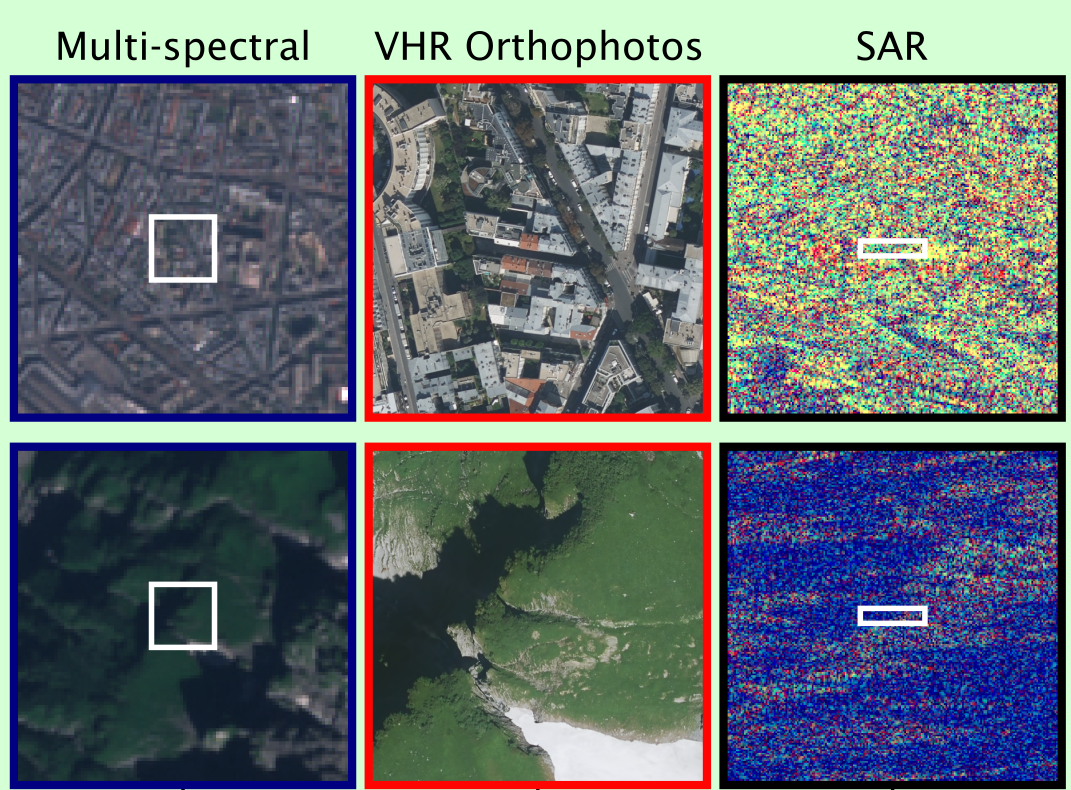
\includegraphics[width=0.85\textwidth]{images/introduction/tammi_graphabstract.png}
\caption{Two example locations imaged by the three modalities used throughout this thesis: Sentinel-2 multispectral, VHR optical (BD ORTHO), and Sentinel-1 SAR. The white rectangle marks the extent of the VHR patch within the wider spatial context covered by the multispectral and SAR imagery, illustrating the nested, multi-resolution relationship between the three modalities discussed below. Reflectance-based imagery (multispectral, VHR) is visually interpretable with some training; SAR backscatter is not, despite encoding genuine information about the scene. Figure from Chapter~\ref{chap:tammi}.}
\label{fig:intro_modality_example}
\end{figure}
 
\textbf{An interactive interface.} Richer sensing data alone does not close the expertise gap described in Section~\ref{sec:intro_extraction_challenge}; it can widen it, since more modalities and bands mean more, not less, specialized interpretation, as Figure~\ref{fig:intro_modality_example} illustrates directly. This thesis instead explores natural language as an interface that allows a user to interact with EO data directly in terms of what they want to know or find, without needing to manually locate, download, and visually interpret imagery themselves. This direction is not specific to remote sensing: it follows from the broader success, on natural images, of models that jointly learn from vision and language, closing part of the gap between a raw visual prediction and the semantic answer a user actually wants. Chapter~\ref{chap:relatedworks} reviews how this general direction has been adapted to remote sensing specifically; here, it is enough to note that three tasks recur throughout that adaptation, and structure this thesis. \textit{Captioning} produces a free-form natural-language description of an image. \textit{Visual question answering} (VQA) addresses the setting where the location of interest is already known: given an image and a question about it, produce an answer. \textit{Retrieval} addresses the inverse setting: given a description of what is being looked for, find the matching locations within a large archive. All three replace manual visual inspection, and the domain expertise it requires, with a natural language query or response; this thesis centers on VQA and retrieval specifically, with captioning appearing as a complementary training signal in Chapter~\ref{chap:multitask}.
 
\section{From Isolated Tasks to Unified Learning}
\label{sec:intro_isolated_unified}
 
RSVQA, the specific instantiation of question answering this thesis studies, has historically been developed as an isolated, single-modality task: a model trained to answer questions about one image, from one sensor, with no other training signal involved. This was, in part, a reasonable starting point: early RSVQA datasets were themselves single-modality, and studying one task on one modality kept the architectural and experimental design tractable while the field established basic feasibility. The first contributions of this thesis (Chapters~\ref{chap:llm_augmentation} and~\ref{chap:seg_attention}) work within this same single-modality setting, improving its robustness and its architecture respectively, before the thesis turns to two ways of moving beyond it.
 
The first is multimodality itself: an analyst's question is rarely answerable from a single sensor alone, as the flood-mapping scenario in Section~\ref{sec:intro_extraction_challenge} illustrates, motivating the combination of VHR, multispectral, and SAR imagery introduced in Section~\ref{sec:intro_multimodal_interactive} within a single RSVQA model (Chapter~\ref{chap:tammi}). The second is task combination: an analyst's needs often span more than question answering alone, encompassing description (captioning), and self-supervised reconstruction requires no annotation at all, only the imagery itself. A natural hypothesis is that training a model on several of these signals jointly, rather than in isolation, produces a shared representation more capable than any single-task model, through two distinct mechanisms: captioning can supply a richer, less templated supervisory signal than question-answering pairs alone, and self-supervised reconstruction can prevent that shared representation from collapsing onto purely semantic features, retaining visual detail a purely discriminative objective might otherwise discard. Whether this hypothesis holds is not, however, something this thesis assumes: Chapter~\ref{chap:multitask} treats it as an empirical question to be tested directly. Retrieval, the second paradigm introduced in Section~\ref{sec:intro_multimodal_interactive}, is not part of this task combination: Chapter~\ref{chap:ctcr} develops it separately.
\section{Scientific Challenges}
\label{sec:intro_challenges}
 
The progression described above, from single-modality RSVQA to multi-modal, multi-task, and retrieval settings, surfaces scientific challenges that structure the contributions of this thesis, and that Chapter~\ref{chap:relatedworks} situates in detail within the broader literature. These challenges fall into four related categories.
 
\textbf{Data-related challenges.} Multi-modal, richly annotated remote sensing datasets remain scarce relative to their natural-image counterparts, a scarcity compounded by the cost and expertise required to annotate imagery correctly, as Section~\ref{sec:intro_extraction_challenge} already established for human interpretation more broadly. Where datasets are generated automatically to work around this cost, as is common practice in RSVQA, the resulting questions are often templated, which risks introducing its own bias: a model can learn to exploit regularities in how questions are phrased rather than the underlying visual reasoning task, a robustness gap distinct from raw accuracy.
 
\textbf{Model-related challenges.} Adapting vision-language architectures developed for natural images to remote sensing is not a direct transfer. RSVQA architectures, for instance, typically compute attention directly from raw visual features, leaving them to jointly discover which regions of an image are relevant and what they mean from question-answering supervision alone, rather than exploiting the structured scene understanding that semantic segmentation already provides as an explicit, separately trainable signal. Handling heterogeneous modalities as different in resolution and physical meaning as VHR optical, multispectral, and SAR imagery, illustrated in Figure~\ref{fig:intro_modality_example}, compounds this further: a model must reconcile inputs that disagree in spatial extent, revisit frequency, and the underlying physical quantity they measure, which has not been systematically addressed at the dataset or architecture level.
 
\textbf{Learning challenges.} Beyond architecture, open questions remain about what a model should be trained to do, and with what supervision. Whether jointly training RSVQA with other tasks measurably improves performance, rather than degrading it, is assumed more often than it is tested; where it has been tested, results are mixed rather than confirmatory, leaving the actual value of multi-task training in this domain an open empirical question rather than a settled premise. Generalizing across sensors and geographic regions, and remaining robust to the kind of linguistic variation noted above, are further instances of the same underlying difficulty: learning representations that hold up outside the narrow conditions a model was trained under.
 
\textbf{Temporal and reasoning challenges.} Finally, most of the settings discussed so far concern a single image at a single point in time. Modeling temporal dynamics, and reasoning jointly over space, time, and language, is comparatively underexplored. Retrieving Earth Observation temporal imagery by composing a visual reference with a textual description of additional change has not previously been formulated as a task, despite its direct operational relevance to change monitoring, where an analyst who has already observed one change pattern often wants to find other locations exhibiting that same pattern together with something further.
 
\section{Research Questions and Thesis Scope}
\label{sec:intro_rq_scope}
 
The four categories of challenge described above raise a single overarching question that this thesis pursues throughout: how can multimodal, language-driven learning improve access to remote sensing information, by jointly leveraging vision and language, addressing data scarcity, exploiting synergies between tasks, and reasoning over space, time, and language together, rather than treating each of these as a separate concern. This thesis pursues that question through five specific research questions, each addressed by one of the contributions previewed in Section~\ref{sec:intro_contributions_overview}:
 
\begin{itemize}
\item \textbf{RQ1}: Can data-centric augmentation improve RSVQA models' robustness to linguistic variation in question phrasing, without sacrificing in-distribution accuracy?
\item \textbf{RQ2}: Does conditioning attention on an explicit semantic segmentation prior improve RSVQA over attention computed from raw visual features alone?
\item \textbf{RQ3}: How can RSVQA be extended to jointly exploit multiple sensing modalities acquired at different spatial resolutions?
\item \textbf{RQ4}: Does training RSVQA jointly with captioning and self-supervised image reconstruction measurably improve either task?
\item \textbf{RQ5}: Can a composed query, combining a visual reference and a textual description, support retrieval of temporal change patterns in Earth Observation archives?
\end{itemize}
 
The scope of this thesis follows directly from these questions. It addresses two language-based interfaces to EO data, question answering and retrieval, rather than the broader space of EO tasks, such as segmentation or detection as standalone goals, that this thesis does not address. The multi-modal and multi-task contributions (Chapters~\ref{chap:tammi} and~\ref{chap:multitask}) are developed and evaluated on datasets covering Metropolitan France, combining VHR, Sentinel-2, and Sentinel-1 imagery specifically; extending this scope geographically, or to further sensing modalities, is discussed as future work in the concluding chapter rather than undertaken here. 
\section{Thesis Contributions Overview}
\label{sec:intro_contributions_overview}
 
This thesis makes six technical contributions, developed across Chapters~\ref{chap:llm_augmentation} through~\ref{chap:ctcr}, each answering one of the five research questions stated in Section~\ref{sec:intro_rq_scope} and grouped into the three stages shown in Figure~\ref{fig:intro_roadmap}: single-modality RSVQA foundations, multi-modal and multi-task RSVQA, and retrieval as a complementary paradigm. Chapter~\ref{chap:relatedworks} first reviews the state of the art across visual question answering, retrieval, and captioning in remote sensing, positioning each contribution below relative to it.
 
\begin{figure}[ht]
\centering
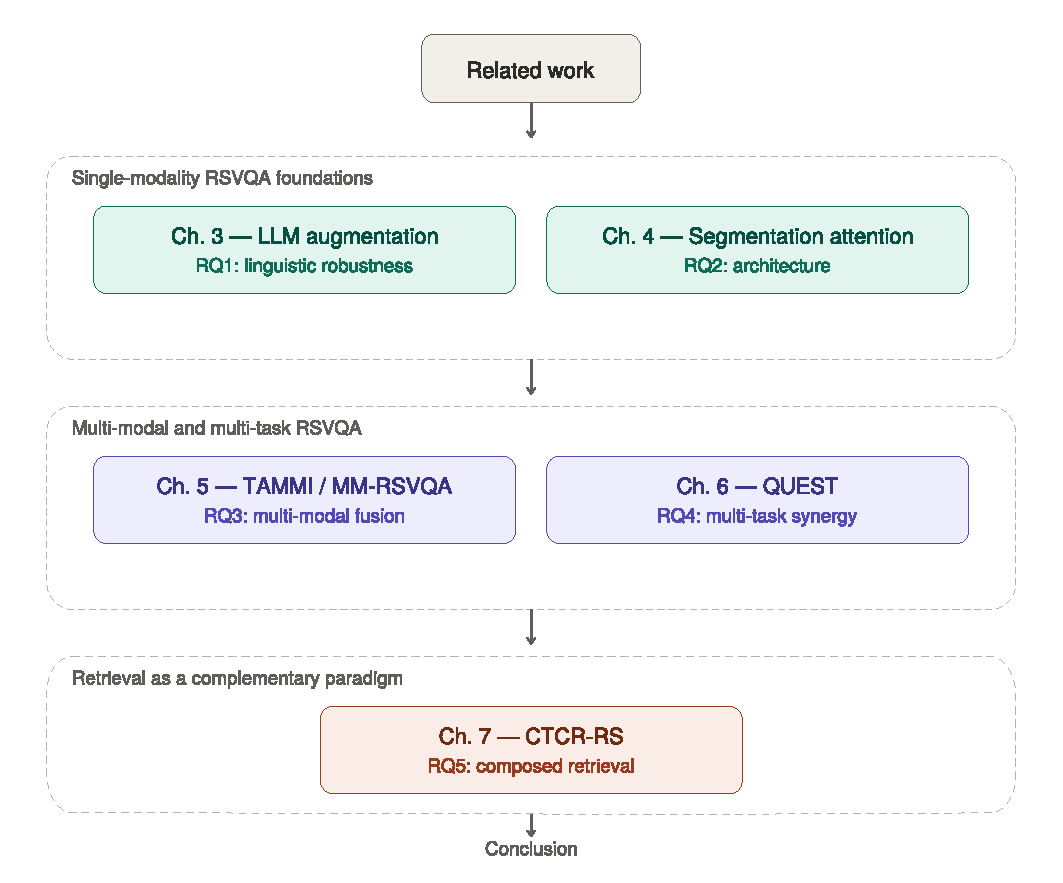
\includegraphics[width=0.85\textwidth]{images/introduction/thesis_roadmap.pdf}
\caption{Roadmap of this thesis's contributions, grouped into the three stages described in Section~\ref{sec:intro_contributions_overview}: single-modality RSVQA foundations (Chapters~\ref{chap:llm_augmentation}-\ref{chap:seg_attention}), multi-modal and multi-task RSVQA (Chapters~\ref{chap:tammi}-\ref{chap:multitask}), and retrieval as a complementary paradigm (Chapter~\ref{chap:ctcr}).}
\label{fig:intro_roadmap}
\end{figure}
 
\textbf{Chapter~\ref{chap:llm_augmentation}} answers RQ1, proposing an LLM-based data augmentation strategy that generates syntactically diverse reformulations of existing training questions, and showing that it improves robustness to unseen phrasings without sacrificing in-distribution accuracy.
 
\textbf{Chapter~\ref{chap:seg_attention}} answers RQ2, proposing a segmentation-guided attention mechanism that conditions the model's attention computation on an explicit, multi-channel semantic segmentation of the scene.
 
\textbf{Chapter~\ref{chap:tammi}} answers RQ3 through two contributions. It introduces TAMMI, a large-scale dataset combining VHR optical, Sentinel-2 multispectral, and Sentinel-1 SAR imagery, establishing multi-modal, multi-resolution VQA as a task in its own right; and MM-RSVQA, a baseline model that fuses all three modalities with the question.
 
\textbf{Chapter~\ref{chap:multitask}} answers RQ4, introducing QUEST, a unified architecture that jointly optimizes reconstruction, captioning, and VQA, and using it to test, rather than assume, whether joint training measurably improves either task.
 
\textbf{Chapter~\ref{chap:ctcr}} answers RQ5, introducing Composed Temporal Change Retrieval (CTCR-RS): given a reference pair of images depicting an observed change and a textual description of an additional change, retrieve archive locations exhibiting the composition of both.
 
The remainder of this thesis is organized as follows. Chapter~\ref{chap:relatedworks} reviews related work across RSVQA, retrieval, and captioning in remote sensing. Chapters~\ref{chap:llm_augmentation} through~\ref{chap:ctcr} present the six contributions summarized above, each structured with its own review of directly relevant related work, methodology, and experimental study. Chapter~\ref{chap:conclusion} concludes the thesis, synthesizing findings across all six contributions and discussing directions for future work.
 